\label {fs-acker-impl}

In the previous section, we introduced a general schema of the \tracker\ framework. In this section, we deepen into its implementation details. We describe and explore the properties of the tracking agent that produces the substream termination notifications (NEOSS). After that, the technique to achieve consistent termination events order is detailed. Distributed implementation of the tracking agent concludes this part.

\subsection{Bound guarantees}

The tracking agent splits the workflow graph into partially ordered segments and track them separately. For each process $p$ we can generate a list of preceding segments that include a set of incoming messages generators $W_p$ for the process. As soon as all these segments contain no elements of a substream the agent sends to a process {\em NEOSS}.

To track the messages path through segments the agent receives SND/RCV reports, that contain a segment identifier and a list of predicates the message satisfies to. The agent aggregates this information into the table illustrated in Table~\ref{tracker-table-simple}.

\begin{table}[htbp]
\caption{\tracker\ table: a general example}
  \label{tracker-table-simple}
  \centering
  \small
  \begin{tabular}{|c|c|c|>{\bfseries}c|} 
    \hline
    Notified & Predicate & Segment & Substream elements  \\ \hline \hline
    \multirow{2}{*}{\checkmark} & \multirow{2}{*}{h(x)} & A & No \\ \cline{3-4}
    & & B & No \\ \hline
    \multirow{2}{*}{} & \multirow{2}{*}{q(x)} & A & No \\ \cline{3-4}
    & & B & Yes \\ \hline
    \multirow{2}{*}{\checkmark} & \multirow{2}{*}{z(x)} & A & No \\ \cline{3-4}
    & & B & No \\ \hline
  \end{tabular}
\end{table}

% A graph shown in Figure~\ref{fig:tracker-acker-comparison} illustrates the notion of segments. This graph has two segments: $A$ and $B$. Note that according to Table~\ref{tracker-table-simple}, the NEOSS for predicate $q(x)$ can be sent for a segment $A$, but not for a segment $B$. This behavior is similar to punctuations: NEOSS can be spawned earlier for the upstream processes.

% \begin{figure}[htbp]
%   \centering
%   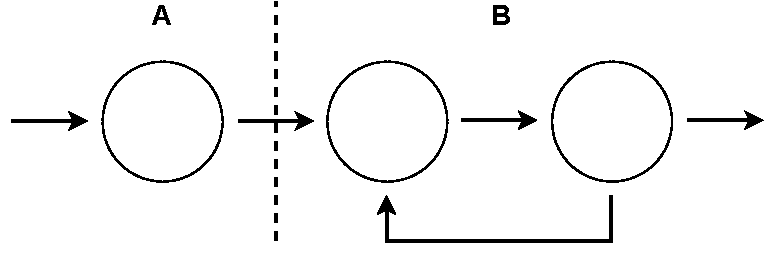
\includegraphics[width=0.3\textwidth]{pics/segments-example.pdf}
%   \caption{Graph segmentation example}
%   \label{fig:tracker-acker-comparison}
% \end{figure}

There are several possible methods to build the indicator that the segment contains elements from a substream using the reports from processes. Our implementation uses the trick applied in Apache Storm to monitor the completeness of processing~\cite{apache:storm:acker}. 

Each report is labeled by a random number $X$, and this number is the same for the send action and the corresponding receive action. This trick makes it easy to check if the segment contains a full set of $SND$/$RCV$ pairs for a message: XOR operation for all numbers received from the chain will turn into 0. The result of the XOR operation can accidentally become zero, but the probability of this event is controlled by the length of the random number $X$ so that it can be neglected in practice~\cite{apache:storm:acker}.

Figure~\ref{fig:tracker-reports} illustrates the reports with random numbers. The elements satisfying a predicate $h(x)$ flow through a dataflow. The first process generates an output and sends the SND report with $X=5$. The corresponding RCV report by the second process also has $X=5$ because this process receives the element from the first one. The second process sends a new element that satisfies $h(x)$ further, and the new SND report with $X=12$ is produced. The third operator receives this element and also produces an RCV report with $X=12$. If there are no more elements such that $h(x)=1$, then we can send NEOSS for the substream defined by $h(x)$ ends because {\em 5 XOR 5 XOR 12 XOR 12 = 0}. 

\begin{figure}[htbp]
  \centering
  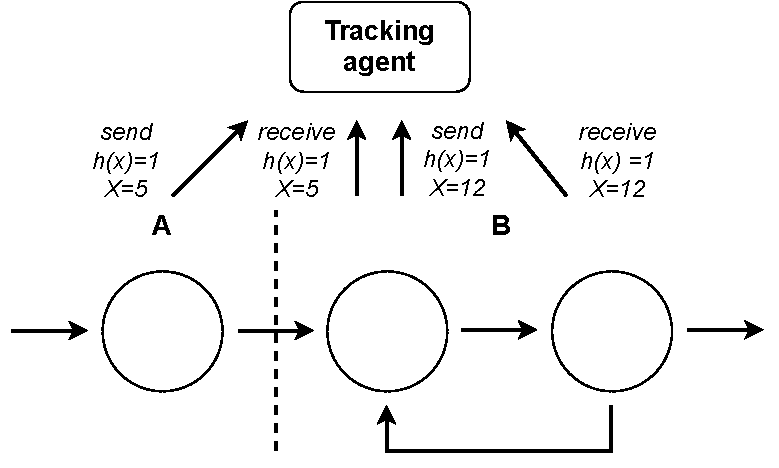
\includegraphics[width=0.3\textwidth]{pics/tracker-segments-example.pdf}
  \caption{Reports example}
  \label{fig:tracker-reports}
\end{figure}

Table~\ref{tracker-table-xor} illustrates the actual \tracker\ table for the mentioned technique.

% All reports from processes are grouped by the satisfying predicate and the segment. Random numbers from these reports are XORed into the result shown in columns {\em Segment XOR} and {\em XOR}. If the XOR value is equal to 0, then the tracking agent can send the NEOSS, providing the soft bound guarantee for the corresponding predicate.

\begin{table}[htbp]
\caption{\tracker\ table: an example with XORing technique}
  \label{tracker-table-xor}
  \centering
  \small
  \begin{tabular}{|c|c|c|>{\bfseries}c|>{\bfseries}c|} 
    \hline
    Notified & Predicate & Segment & Segment XOR & XOR  \\ \hline \hline
    \multirow{2}{*}{\checkmark} & \multirow{2}{*}{h(x)} & A & 000 & \multirow{2}{*}{000} \\ \cline{3-4}
    & & B & 000 & \\ \hline
    \multirow{2}{*}{} & \multirow{2}{*}{q(x)} & A & 000 & \multirow{2}{*}{110} \\ \cline{4-4}
    & & B & 110 & \\ \hline
    \multirow{2}{*}{\checkmark} & \multirow{2}{*}{z(x)} & A & 000 & \multirow{2}{*}{000} \\ \cline{3-4}
    & & B & 000 & \\ \hline
  \end{tabular}
\end{table}

Due to the associativity of XOR, we can optimize tracking agent incoming traffic by aggregating reports locally within the processes. For each process, we introduce a {\em local tracking agent} component. It serves as a mediator between the process and the global agent, buffering the outgoing reports and flushing them periodically. 

The flushing window is the parameter that allows us to balance between the service traffic and latency between the actual substream termination (the event from data producer) and termination event. Note that substreams last a finite time period by definition, so we assume that each process sends aggregated reports a constant number of times that does not depend on the number of substreams and processes. Therefore, the amount of extra network traffic for the reports is $O(|\Pi|)$, so the total estimation with the overhead on the notifications is $O(K|\Pi|)$.

\subsection{Consistent termination events order}

If the order of NEOSS is consistent, the order of termination events will be consistent as well. To achieve consistent order of NEOSS, we need to define $t(M)$ such that the order on $t(M)$ respects the order of input elements. All reports that processes send to the tracking agent should be labeled with $t(M)$. In turn, the tracking agent sends the NEOSS elements according to the order on $t(<)$.

Table~\ref{tracker-table-oder} illustrates the \tracker\ table in case of consistent NEOSS order. Column {\em min t(x)} indicates the minimal $t(x)$ among the elements that satisfy the corresponding predicate. The tracking agent sends notifications for the substream if the $XOR$ value is 0 and all substreams that contain elements with less {\em min t(x)} have finished (notifications have been produced). Therefore, NEOSS for the substream defined by the predicate $h(x)$ is not sent until the NEOSS for the predicate $q(x)$ is generated. 

\begin{table}[htbp]
\caption{\tracker\ table: an example with consistent NEOSS order}
  \label{tracker-table-oder}
  \centering
  \small
  \begin{tabular}{|c|c|>{\bfseries}c|c|} 
    \hline
    Notified & Predicate & min t(x) &  XOR  \\ \hline \hline
    \multirow{2}{*}{waits for q(x) finish} & \multirow{2}{*}{h(x)} & \multirow{2}{*}{5} & \multirow{2}{*}{000} \\
    & & & \\ \hline
    \multirow{2}{*}{} & \multirow{2}{*}{q(x)} & \multirow{2}{*}{4} & \multirow{2}{*}{110} \\
    & & & \\ \hline
    \multirow{2}{*}{\checkmark} & \multirow{2}{*}{z(x)} & \multirow{2}{*}{1} & \multirow{2}{*}{000} \\
    & & & \\ \hline
  \end{tabular}
\end{table}

If input elements arrive through a single node, $t(x)$ can denote the monotonic system time of the element $x$ arrival. If there are multiple source processes, one can use time oracle agent~\cite{10.14778/3055330.3055335} as a service for generation a monotonic sequence of unique timestamps. However, in this case, there is a need to manage one more subsystem.

A simple technique to build $t(x)$ without extra agents bases on systematic synchronization of the system clocks. We call this method and associated labels {\em coarse time}. Assume that clock differences are no more than some fixed $\delta$, which we reference as synchronization slack. Let $\tau(x)$ be precise physical time of input data item $x$ arrival, and $s(x)$ be local system time of the source node where $x$ arrived. The true order of events $\tau(d_1) > \tau(d_2)$ coming from different sources can be sometimes restored by their system timestamps $s(d_1)$ and $s(d_2)$. If these timestamps differ more than time synchronization slack, then the order is clear: $s(d_1) > s(d_2) + \delta \Rightarrow \tau(d_1) > \tau(d_2)$.

This fact allows us to define $t(x)$ such that $t(x) = [s(x) / \delta]$. This way we make $t(x)$ less precise, but this trick gives us an ability to compare global time associated by different source nodes. If $t(x_1)$ is greater than the $(t(x_2) + 1)$ then their order is defined even if they arrived from different source nodes:  $t(x_1) > t(x_2) + 1 \Rightarrow \tau(x_1) > \tau(x_2)$. Therefore, the order on $t(x)$ coincides with the order of input elements, so it is suitable for the defined problem. Here is a summary of the mechanism that ensures consitent termination events order:
\begin{enumerate}
    \item On input item arrival, source node gets the system timestamp
    \item The system timestamp is shrunk up to synchronization slack (practically we achieve 10ms slack)
    \item Each report for the tracking agent is labeled by the result of $t(x)$
    \item Tracking agent sends NEOSS according to the order on $t(x)$
    \item Termination events are generated according to the order of NEOSS arriving
\end{enumerate}

\subsection{Distributed tracking agent}

The tracking agent accumulates all the service traffic from the entire system. To ensure scalability, we introduce a distributed version of the tracking agent.

A straightforward approach is to partition predicates between the shards of the tracking agent. For example, one shard can handle all reports for the predicate $h(x)$, while the second all reports for the predicate $q(x)$. Note that the network traffic complexity remains the same $O(K|\Pi|)$ because each process sends each report to only a single shard depending on the predicate.

The main problem regarding this approach is to enforce the consistent NEOSS order. Centralized agent sends NEOSS through the FIFO network channels, so the NEOSS elements for the same processes cannot be reordered. There can be a race between NEOSS from various shards due to asynchronous network channels in the distributed case.

A simple solution for this issue is on each NEOSS from some shard, wait for NEOSS from all other shards, but with greater $t(x)$. For example, if a process receives NEOSS for some predicate with $\min t(x) = 3$, then it needs to wait until receiving NEOSS with $t(x) > 3$ from all other shards to produce the termination event. However, this method can increase the latency between the substream end and the termination event.

We employ the vector clock algorithm to mitigate latency overhead. Each process either periodically sends its system time to all tracking agent shards. In turn, tracking agents also periodically sends the minimal vector among the in-flight elements. Therefore, if a process receives NEOSS for some predicate with $\min t(x) = 3, vec=[0,4,1]$, then it needs to wait until receiving of vectors component-wise greater than $[0,4,1]$ from all shards to produce the termination event.

The vector clock introduction increases the service traffic but allows to eliminate bottleneck from the system. The service traffic complexity remains the same, but the $O$ factor increases. In the experimental section, we will study how significant is this increase.

